% !TEX root = ../main.tex
\subsection{Fiducial Cuts}
\label{20.02::fiducial_cuts}
    % What are fiducial cuts?
    In detector physics, the fiducial region is defined as the region considered reliable and suitable for analysis.
    Fiducial cuts are constraints applied to experimental data in order to define this region.
    Thus, they allow us to exclude events or measurements that may be affected by experimental artefacts, detector inefficiencies, or other factors that could introduce systematic errors and biases \cite{leo1987}.

    % Why weren't fiducial cuts used in this thesis?
    Due to its 6-sector geometry, fiducial cuts are of particular importance for CLAS12 FD analysis.
    However, they were disregarded for this particular study.
    This is because of its broadness: we are only concerned with the phase space of DIS variables and the general statistics, as detailed in Section \ref{14.30::study_results}.
    While the cuts would likely improve the quality of the results, the data is broad enough to be considered resilient to the damage of not applying them.

    % How would we implement them?
    To apply such cuts, we would need to follow the procedure described in \cite{zana2010}.
    This would involve providing $\phi$ vs $\theta$ curves that cut all events at the edges of each DC sector.
    One curve would be needed for each $p$ bin, for each sector.
    Finally, different curves would be needed for each PID being processed.

    % Show plots.
    Examples of $\phi$ vs $\theta$ distributions for different $p$ bins can be seen in Figures \ref{fig::20.02::fiducial_cuts_pid11}, \ref{fig::20.02::fiducial_cuts_pid211}, and \ref{fig::20.02::fiducial_cuts_pid-211}, where we show the distributions for $e^-$, $\pi^+$, and $\pi^-$.
    As can be seen in the plots, the separation between the DC's areas and its edges are easily observed in a layer-by-layer basis.

    % e-.
    \begin{figure}[b!]
        \centering
        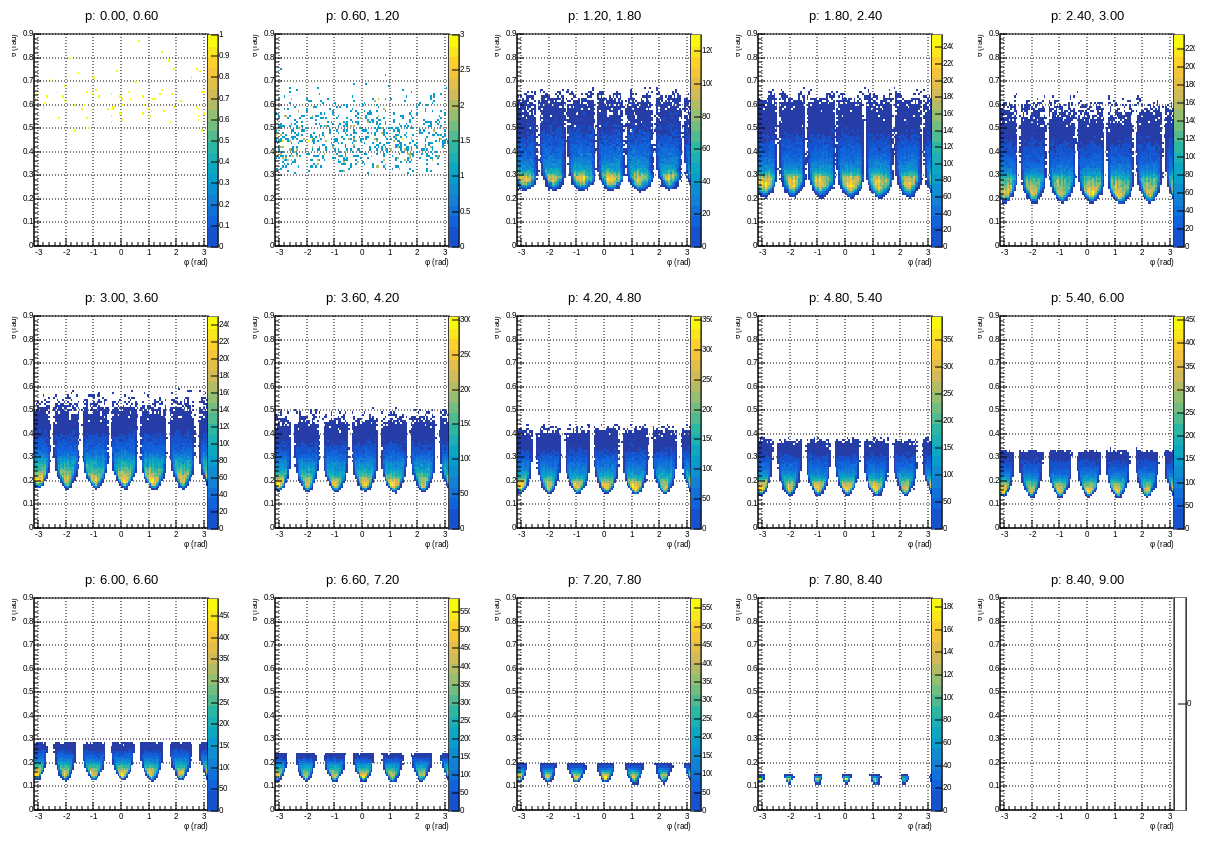
\includegraphics[width=\textwidth]{02fidcuts_11.png}
        \caption[$\phi$ vs $\theta$ of $e^-$ in $p$ bins]
        {$\phi$ vs $\theta$ of $e^-$ detected by DC, separated in $p$ bins.
        Run 12016.}
        \floatfoot{Source: Own elaboration, using the \href{https://github.com/bleaktwig/clas12-rge-analysis}{clas12-rge-analysis} software.}
        \label{fig::20.02::fiducial_cuts_pid11}
    \end{figure}

    \begin{figure}
        % pi+.
        \begin{subfigure}[b]{\textwidth}
            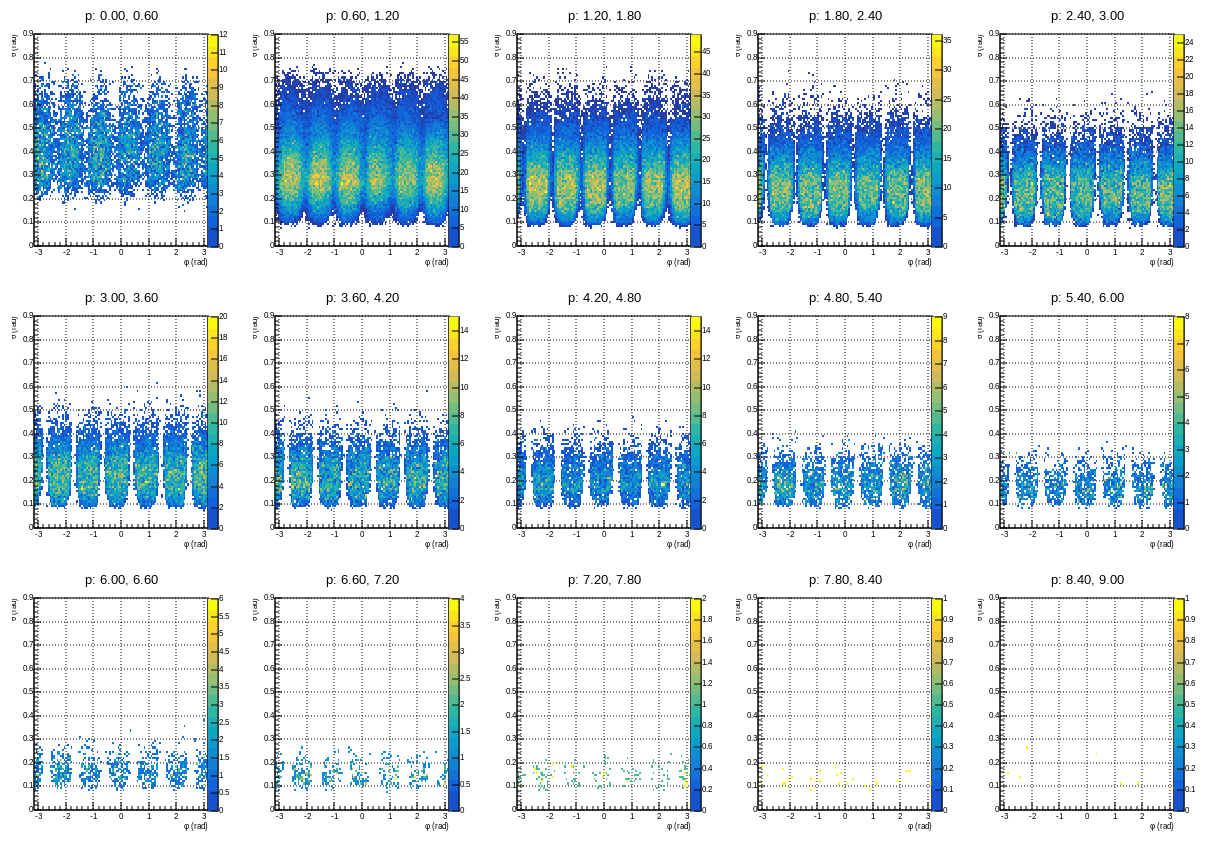
\includegraphics[width=\textwidth]{02fidcuts_211.png}
            \caption{$\phi$ vs $\theta$ of $\pi^+$.}
            \label{fig::20.02::fiducial_cuts_pid211}
        \end{subfigure}
        % pi-.
        \begin{subfigure}[b]{\textwidth}
            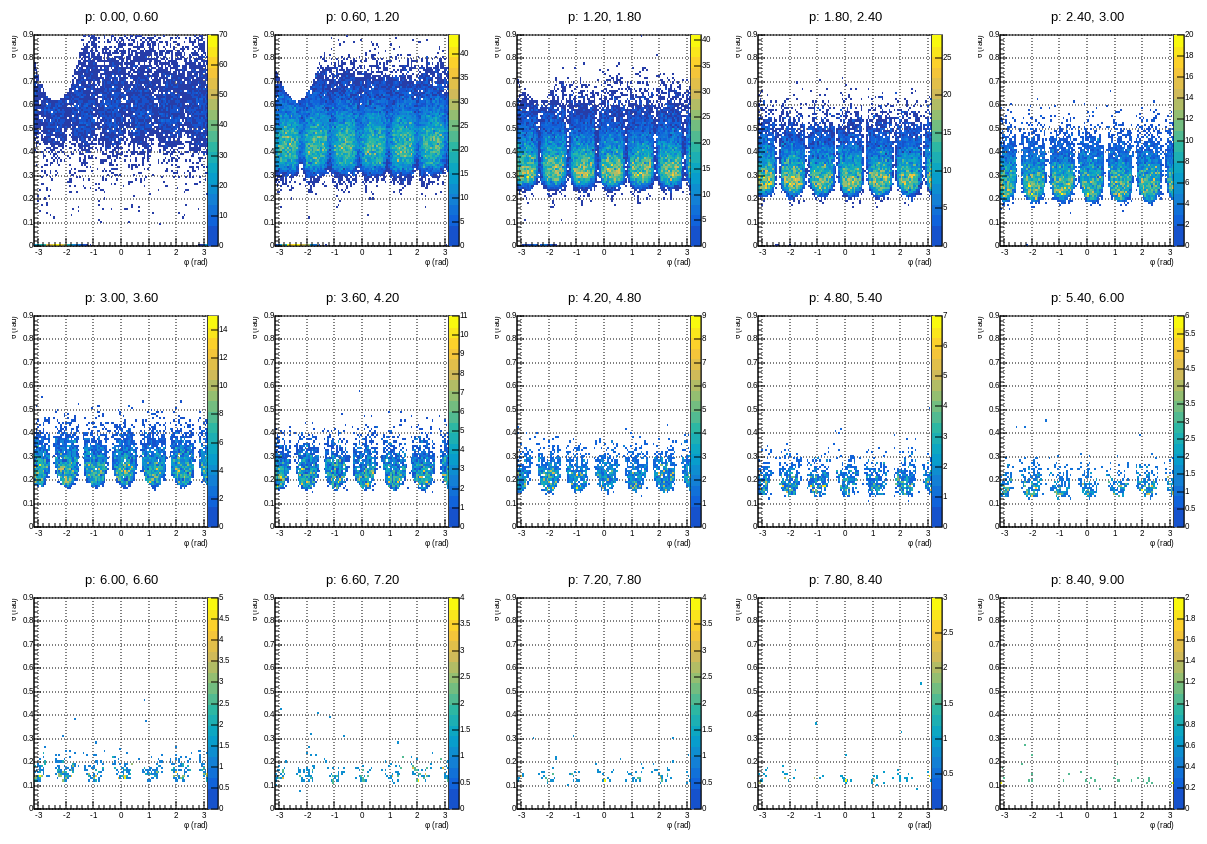
\includegraphics[width=\textwidth]{02fidcuts_-211.png}
            \caption{$\phi$ vs $\theta$ of $\pi^-$.}
            \label{fig::20.02::fiducial_cuts_pid-211}
        \end{subfigure}

        \caption[$\phi$ vs $\theta$ of $\pi^+$ and $\pi^-$, separated in $p$ bins.]
        {$\phi$ vs $\theta$ of $\pi^+$ and $\pi^-$ detected by DC, separated in $p$ bins.
        Run 12016.}
        \floatfoot{Source: Own elaboration, using the \href{https://github.com/bleaktwig/clas12-rge-analysis}{clas12-rge-analysis} software.}
        \label{fig::20.02::fiducial_cuts_pions}
    \end{figure}

    \pagebreak
